\documentclass[xcolor=pdftex,romanian,colorlinks]{beamer}
%\documentclass[xcolor=pdftex,handout,romanian,colorlinks]{beamer}

\usepackage[export]{adjustbox}
\usepackage{../sty/tslides}
\usepackage[all]{xy}
\usepackage{pgfplots}
\usepackage{flowchart}
\usepackage{todonotes}
\usetikzlibrary{arrows,positioning,calc}
\lstset{language=Haskell}
\lstset{escapeinside={(*@}{@*)}}
\PrerenderUnicode{ăĂîÎȘșȚțâÂ}

%\usepackage{xcolor}
%\definecolor{IntensColor}{HTML}{2E86C1}
%\definecolor{StateTransition}{HTML}{D6EAF8}
%\definecolor{MedianLightOrange}{RGB}{216,178,92}
%\definecolor{Orchid}{HTML}{8E44AD}
%\definecolor{True}{HTML}{229954}
%\definecolor{False}{HTML}{CB4335}


\usepackage{proof}
\usepackage{multirow}
\usepackage{alltt}
\usepackage{mathpartir}
\usepackage{ulem}

\newcommand{\structured}[1]{#1}

\definecolor{IntensColor}{HTML}{2E86C1}
\definecolor{StateTransition}{HTML}{D6EAF8}
\definecolor{MedianLightOrange}{RGB}{216,178,92}
\definecolor{Orchid}{HTML}{8E44AD}
\definecolor{True}{HTML}{229954}
\definecolor{False}{HTML}{CB4335}

\newcommand{\cin}[1]{{\color{cobalt} #1}}
\newcommand{\sel}[1]{{\color{Orchid} #1}}

\newcommand{\intens}[1] {{\color{IntensColor} #1}}
\newcommand{\exe}[1] {{\color{True} #1}}

\newcommand{\la}{\lambda}

\setlength{\leftmargini}{0pt}

\newcommand{\app}[2]{#1\, #2}
\newcommand{\abs}[2]{\lambda #1.\,#2}

\newcommand{\type}[2]{{\color{True}#1\hspace{-.05cm}:}\,{\color{Orchid}#2}}

\newcommand{\sub}[3]{#1\langle#2/#3\rangle}
\newcommand{\subt}[3]{#1[#2/#3]}
\newcommand{\equiva}{=_\alpha}

\newcommand{\trueL}{\mathbf{T}}
\newcommand{\falseL}{\mathbf{F}}
\newcommand{\notL}{\mathbf{not}}
\newcommand{\andL}{\mathbf{and}}
\newcommand{\orL}{\mathbf{or}}
\newcommand{\ifL}{\mathbf{if}}
\newcommand{\boolL}{\mathbf{bool}}

\newcommand{\maybeL}{\mathbf{maybe}}
\newcommand{\nothingL}{\mathbf{Nothing}}
\newcommand{\justL}{\mathbf{Just}}
\newcommand{\Maybe}[1]{\mathop{\mathbf{Maybe}}{#1}}

\newcommand{\foldrL}{\mathbf{foldr}}
\newcommand{\nilL}{\mathbf{Nil}}
\newcommand{\consL}{\mathbf{Cons}}
\newcommand{\ListL}[1]{\mathop{\mathbf{List}}{#1}}

\newcommand{\unpairL}{\mathbf{uncons}}
\newcommand{\pairL}{\mathbf{Pair}}
\newcommand{\firstL}{\mathbf{first}}
\newcommand{\secondL}{\mathbf{second}}
\newcommand{\Pair}[2]{\mathop{\mathop{\mathbf{Pair}}{#1}}{#2}}

\newcommand{\succL}{\mathbf{Succ}}
\newcommand{\zeroL}{\mathbf{Zero}}
\newcommand{\iterateL}{\mathbf{iterate}}
\newcommand{\addL}{\mathbf{add}}
\newcommand{\mulL}{\mathbf{mul}}
\newcommand{\expL}{\mathbf{exp}}
\newcommand{\isZero}{\mathbf{isZero}}
\newcommand{\pred}{\mathbf{pred}}
\newcommand{\factL}{\mathbf{fact}}

\newcommand{\BoolT}{\ensuremath{\texttt{Bool}}}
%\newcommand{\BoolT}{\ensuremath{\texttt{Bool}}}
\newcommand{\ifT}[3]{\mathrm{if}\ #1\ \mathrm{then}\ #2\ \mathrm{else}\ #3}

\newcommand{\UnitT}{\ensuremath{\texttt{Unit}}}
\newcommand{\unit}{\mathrm{unit}}

\newcommand{\VoidT}{\ensuremath{\texttt{Void}}}
\newcommand{\void}{\mathrm{void}}


\newcommand{\ProductT}[2]{#1 \times #2}
\newcommand{\PairL}[2]{\langle #1,#2\rangle}
\newcommand{\ProjOne}[1]{fst\ #1}
\newcommand{\ProjTwo}[1]{snd\ #1}

\newcommand{\SumT}[2]{#1 + #2}
\newcommand{\Left}[1]{\mathrm{Left}\ #1}
\newcommand{\Right}[1]{\mathrm{Right}\ #1}
\newcommand{\Case}[3]{\mathrm{case}\ #1\ \mathrm{of}\ #2\ ;\ #3}

%----------------------------------------------

\newcommand{\SSnot}{\terminal{not}}

\newcommand{\Sand}{\terminal{and}}
\newcommand{\Sor}{\terminal{or}}
\newcommand{\Splus}{\terminal{+}}
\newcommand{\Smul}{\terminal{*}}
\newcommand{\Ssucc}{\terminal{S}}
\newcommand{\Spow}{\terminal{pow}}
\newcommand{\Spred}{\terminal{pred}}
\newcommand{\Seq}{\terminal{eq}}
\newcommand{\Sneq}{\terminal{neq}}

\newcommand{\SisZero}{\terminal{isZero}}
\newcommand{\Slte}{\terminal{<=}}
\newcommand{\Sgte}{\terminal{>=}}
\newcommand{\Slt}{\terminal{<}}
\newcommand{\Sgt}{\terminal{>}}
\newcommand{\Spair}{\terminal{pair}}
\newcommand{\Sfst}{\terminal{fst}}
\newcommand{\Ssnd}{\terminal{snd}}
\newcommand{\Sminus}{\terminal{-}}

\newcommand{\Snull}{\terminal{null}}
\newcommand{\Scons}{\terminal{cons}}
%\newcommand{\c sead}{\terminal{head}}
\newcommand{\SisNull}{\terminal{?null}}
\newcommand{\Stail}{\terminal{tail}}
\newcommand{\Ssum}{\terminal{sum}}
\newcommand{\Sfoldr}{\terminal{foldr}}
\newcommand{\Smap}{\terminal{map}}
\newcommand{\Sfilter}{\terminal{filter}}

\newcommand{\const}[1]{\triangleright {\color{False} #1}}

\newcommand{\egf}[1]{\stackrel{\cdot}{=}_{#1}}

\newcommand{\Conf}[2]{\ensuremath{\langle #1\ ,\ #2\rangle}}
\newcommand{\plus}[1] {{\color{True} #1}}
\newcommand{\te}[1]{\mbox{\texttt{#1}}}

\newcommand{\vexp}{\ensuremath{\mathbb{E}}}
\newcommand{\bexp}{\ensuremath{\mathbb{B}}}
\newcommand{\cmd}{\ensuremath{\mathbb{C}}}

\definecolor{section-color}{HTML}{23373b} %mDarkTeal
%\AtBeginSection[]{
%  \begin{frame}
%  \vfill
%  \centering
%  \begin{beamercolorbox}[sep=8pt,center,shadow=true,rounded=true]{title}
%    \usebeamerfont{title}\insertsectionhead\par%
%  \end{beamercolorbox}
%  \vfill
%  \end{frame}
%}


\title[FLP]{Fundamentele limbajelor de programare}
\subtitle{C01}
\date{}


\begin{document}
\begin{frame}
  \titlepage
\end{frame}

%================================================
\section{\color{section-color} Organizare}
%================================================

\begin{frame}{Instructori}
\begin{itemize}
	\item \intens{Curs}
	\begin{itemize}
		\item Seria 23: Traian Șerbănuță
		\item Seria 24: Denisa Diaconescu
		\item Seria 25: Traian Șerbănuță
	\end{itemize}
	\vspace{.2cm}
	\item \intens{Laborator}
	\begin{itemize}
		\item 231: Horațiu Cheval
		\item 232: Horațiu Cheval/Bogdan Macovei
		\item 233: Andrei V\u acaru
		\item 234: Horațiu Cheval/Bogdan Macovei
		\item 241: Natalia Ozunu
		\item 242: Bogdan Macovei
		\item 243: Bogdan Macovei
		\item 244: Bogdan Macovei
		\item 251: Mihai Calancea
		\item 252: Andrei Burdușa
	\end{itemize}
\end{itemize}
\end{frame}

%------------------------------------------------

\begin{frame}{Resurse}
\begin{itemize}
	\item Moodle 
	\vspace{.2cm}
	\item Teams \\ \intens{\url{https://tinyurl.com/FLP2023-Teams}}
	\vspace{.2cm}
	\item Suporturile de curs si laborator \\ \intens{\url{https://tinyurl.com/FLP2023-Materials}}
\end{itemize}
\end{frame}

%------------------------------------------------

\begin{frame}{Prezență}

Prezența la curs sau la laboratoare nu este obligatorie, \\dar extrem de încurajată.

%\vspace{.2cm}
%In limita locurilor disponibile, puteti sa mergeți la orice curs/laborator. Veți fi expusi la aceeasi informatie.

\end{frame}
%------------------------------------------------

\begin{frame}{Evaluare}
\begin{block}{Notare}
\begin{itemize}
\item \intens{Nota finală:} 1 (oficiu) + nota laborator + parțial + examen 
\item \intens{Restanță:} 1 (oficiu) +  examen \\ (nota de la laborator si parțialul nu se iau în calcul la restanță) 
\end{itemize}
\end{block}


\begin{block}{Condiție de promovabilitate}
\begin{itemize}
\item  \alert{cel puțin 5} > 4.99
\end{itemize}
\end{block}
\end{frame}

%------------------------------------------------
\begin{frame}{Nota laborator}
\begin{itemize}
	\item valorează \intens{2 puncte} din nota finală
	\item se notează activitatea din cadrul laboratorului
	%\item se acorda 1 punct pe activitatea din saptamanile 1-6 (prima parte a laboratorului) si 1 punct pe activitatea din saptamanile 8-14 (a doua parte a laboratorului) 
\end{itemize}
\end{frame}

%------------------------------------------------
\begin{frame}{Examen parțial}
\begin{itemize}
	\item valorează \intens{3 puncte} din nota finală
	\item durata 30 min
	\item în săptămâna 7, în cadrul cursului
	\item nu este obligatoriu și nu se poate reface
	\item întrebări grilă asemănatoare cu cele din quiz-urile de la curs 
	\item materiale ajutătoare: suporturile de curs și de laborator
\end{itemize}
\end{frame}

%------------------------------------------------
\begin{frame}{Examen final}
\begin{itemize}
	\item valorează \intens{4 puncte} din nota finală
	\item durata 1 oră
	\item în sesiune, fizic
	\item acoperă toată materia
	\item exerciții asemănătoare cu exemplele de la curs (nu grile)
	\item materiale ajutătoare: suporturile de curs și de laborator
\end{itemize}
\end{frame}
%------------------------------------------------


%------------------------------------------------

\begin{frame}{Imagine de ansamblu asupra materiei}
 
\begin{columns}
\begin{column}{.5\textwidth}
\intens{Curs}
\begin{itemize}
	\item \alert{Partea I}
	\begin{itemize}
		\item Lambda calcul
		\item Deducție naturală
		\item Corespondența Curry-Howard
	\end{itemize}
	\item \alert{Partea II}
	\begin{itemize}
		\item Puncte fixe/recursivitate
		\item Semantica limbajelor de programare
		\item Elemente de programare logică*
	\end{itemize}
\end{itemize}
\end{column}
\begin{column}{.5\textwidth}

\vspace{-2.2cm}
\intens{Laborator}
\begin{itemize}
		\item Limbajul suport: Haskell
		\item Parsere
		\item Type-checking 
		\item Implementarea unor semantici de limbaje
	%	\item Limbajul suport: Prolog
	%\end{itemize}
\end{itemize}
\end{column}
\end{columns}
\end{frame}

%------------------------------------------------
\begin{frame}{Bibliografie}

{\footnotesize
\begin{itemize}
\item H. Barendregt, E. Barendsen, {\bf Introduction to Lambda Calculus}, 2000.
\item R. Nederpelt, H. Geuvers , {\bf Type Theory and Formal Proof}. Cambridge University Press, 2014.
\item B.C. Pierce,  {\bf Types and programming languages}. MIT Press, 2002
\item P. Selinger,{\bf Lecture Notes on the Lambda Calculus}. Dep. of Mathematics and Statistics, Dalhousie University, Canada.
\item P. Blackburn, J. Bos, and K. Striegnitz, {\bf Learn Prolog Now!} (Texts in Computing, Vol. 7),College Publications, 2006
\item M. Huth, M. Ryan, {\bf Logic in Computer Science (Modelling and Reasoning about Systems)}, Cambridge University Press, 2004.
\item J. Lloyd. {\bf Foundations of Logic Programming}, second edition. Springer, 1987.
%\item G. Winskel,  {\bf The formal semantics of programming languages}. MIT Press. 1993
\end{itemize}
}
\end{frame}

%-------------------------------------------------------
\begin{frame}{La acest curs vom folosi destul de mult literele grecești}
 
\begin{center}
\vspace{-.6cm}

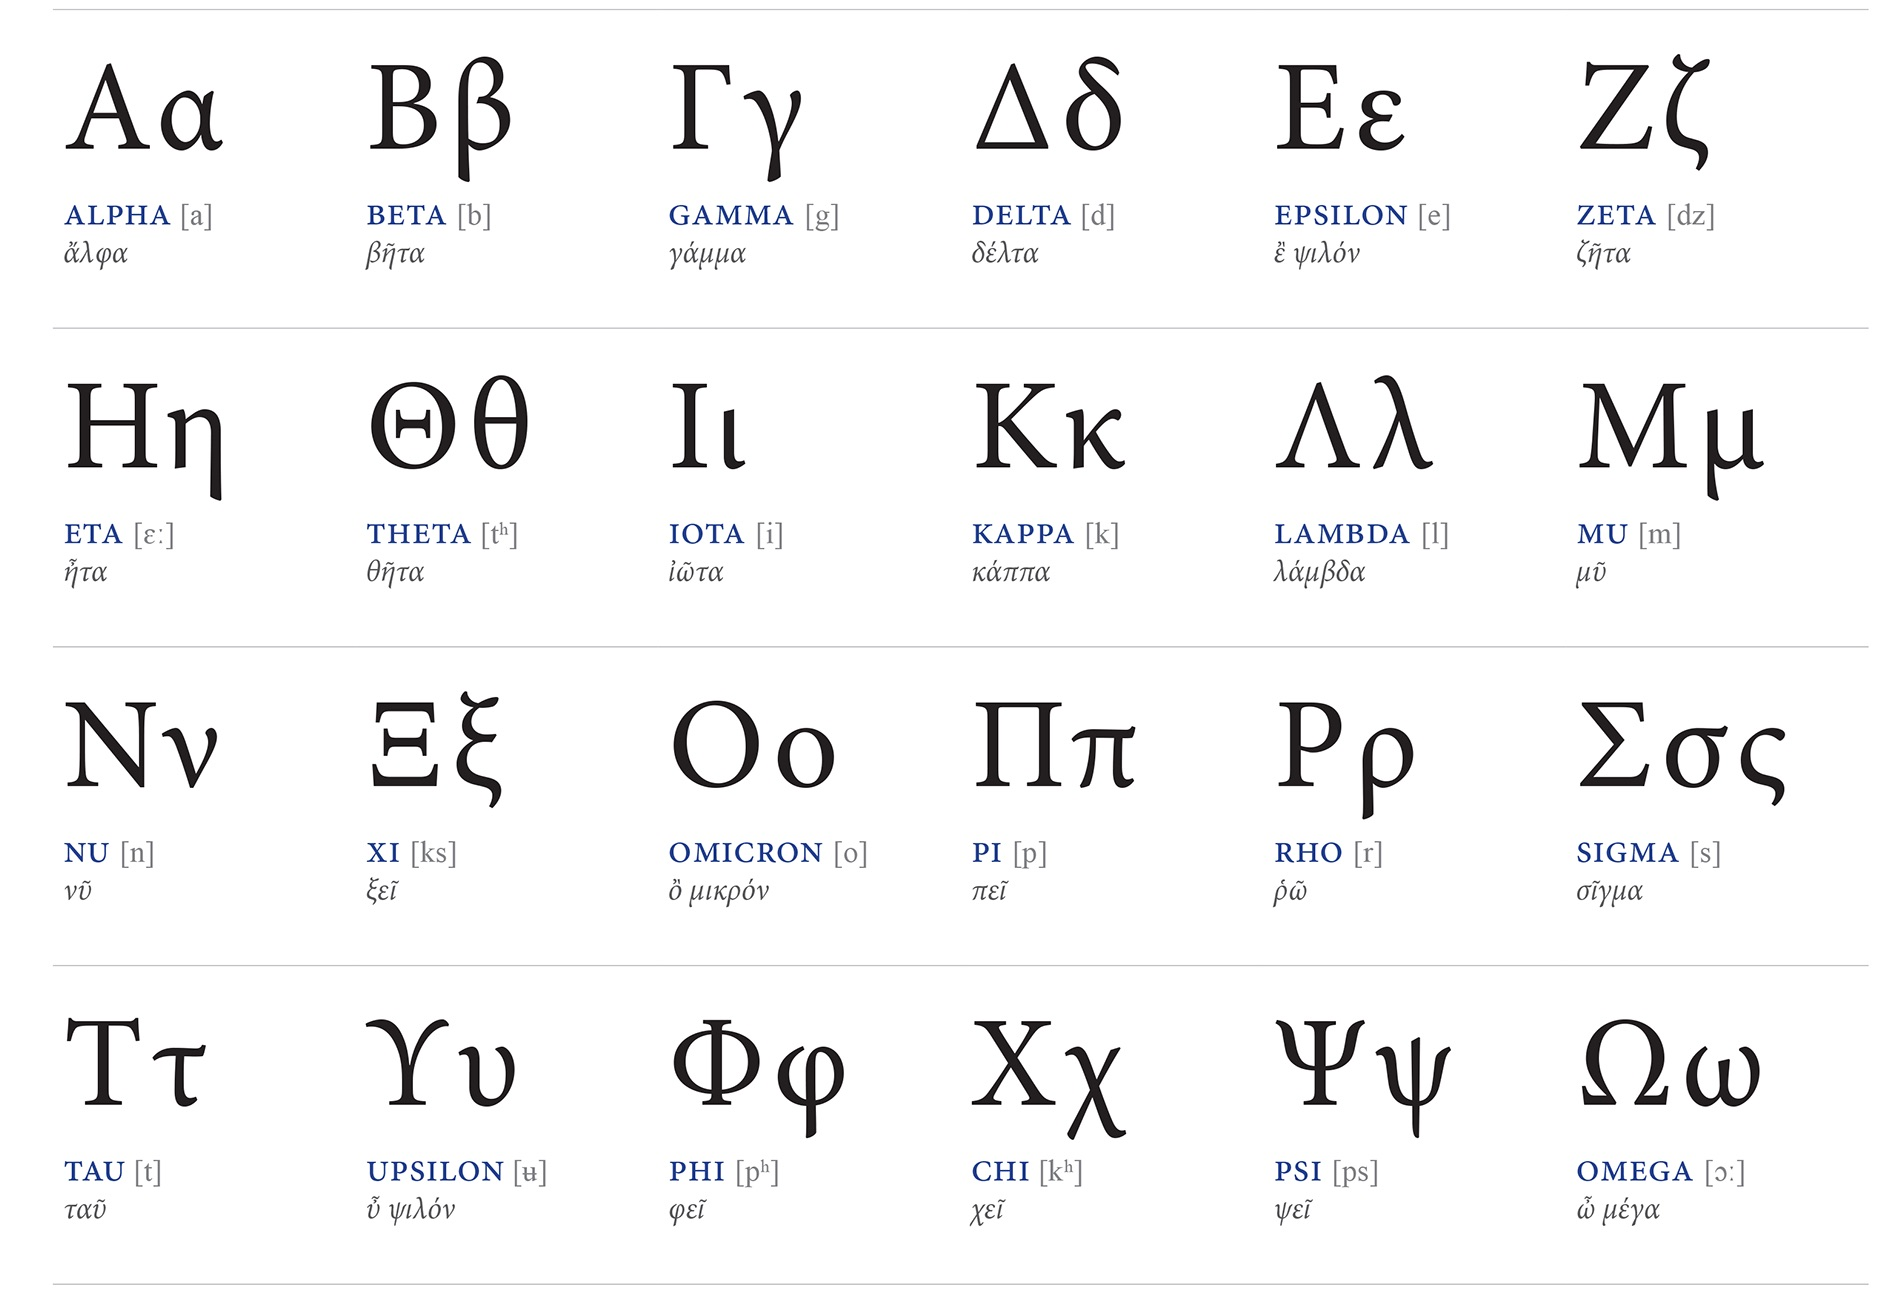
\includegraphics[scale=.17]{images/GreekAlphabet}
\end{center}
 
 
 \end{frame}

%-------------------------------------------------------
\begin{frame}{Integritate academică}

\begin{center}
{\Large \alert{\textbf{Nu trișați, cereți-ne ajutorul!}}}


\bigskip

\includegraphics[scale=.4]{images/Dishonesty.jpg}
\end{center}

\end{frame}

%================================================
\section{\color{section-color} Ce și de ce lambda calcul?}
%================================================


%------------------------------------------------
\begin{frame}{Ce este o funcție în matematică?}

\begin{itemize}
\item In matematica modernă, avem \intens{"funcții prin grafice"}:
\begin{itemize}
	\item orice funcție $f$ are un \alert{domeniu $X$} și un \alert{codomeniu $Y$} fixate, și
	\item orice funcție $f : X \to Y$ este o \alert{mulțime de perechi $f \subseteq X \times Y$} a.î. pentru orice $x \in X$, există exact un $y \in Y$ astfel încât $(x,y)\in f$. 
\end{itemize}

\medskip
\item Acesta este un punct de vedere \intens{\textit{extensional}},  singurul lucru pe care îl putem observa despre funcție este cum duce intrările în ieșiri.

\medskip
\item Două funcții $f,g : X \to Y$ sunt considerate ca fiind \intens{\textit{extensional} egale} dacă pentru aceeași intrare obțin aceeași ieșire,
\begin{center}
$f(x) = g(x)$, pentru orice $x \in X$.
\end{center}
\end{itemize}
\end{frame}

%------------------------------------------------
\begin{frame}{Ce este o funcție în matematică?}

\begin{itemize}
\item Înainte de secolul 20, funcțiile erau privite ca \intens{"reguli/formule"}. 

\medskip
\item A defini o funcție înseamnă să dai  o regulă/formulă pentru a o calcula.
De exemplu,
\begin{center}
\exe{$f(x) = x^2 - 1$}.
\end{center}  

\medskip
\item Doua funcții sunt \intens{\textit{intensional} egale}  dacă sunt definite de aceeași formulă. De exemplu, este f de mai sus  intensional egala cu g de mai jos?
\begin{center}
\exe{$g(x) = (x - 1)(x + 1)$}.
\end{center}

\medskip
\item Daca privim o funcție ca o formulă, nu este mereu necesar să știm domeniul și codomeniul ei. De exemplu, funcția identitate
\begin{center}
\exe{$h(x) = x$}
\end{center}  
poate fi privită ca o funcție $h : X \to X$, pentru orice mulțime $X$.
\end{itemize}
\end{frame}

%------------------------------------------------
\begin{frame}{Extensional vs. intensional}

\begin{itemize}
\item Paradigma \intens{"funcții prin grafice"} este foarte elegantă și definește o clasă mai largă de funcții, deoarece cuprinde și funcții care nu pot fi definite prin formule.

\medskip
\item Paradigma \intens{"funcții ca formule"} este utilă de multe ori în informatică. De exemplu, putem privi un program ca o funcție de la intrări la ieșiri. De cele mai multe ori, nu ne interesează doar cum sunt duse intrările în ieșiri, ci și cum o putem implementa, cum a fost calculată ieșirea, diverse informații suplimentare etc.
\begin{itemize}
	\item Cât a durat să o calculăm?
	\item Câtă memorie a folosit?
	\item Cu cine a comunicat?
\end{itemize}
\end{itemize}
\end{frame}

%------------------------------------------------
\begin{frame}{O paranteză: expresii aritmetice}

\begin{itemize}
\item \intens{Expresiile aritmetice} sunt construite din
\begin{itemize}
	\item variabile ($x, y, z, \ldots$)
	\item numere ($1, 2, 3, \ldots$)
	\item operatori ("$+$", "$-$", "$\times$" etc)
\end{itemize}

\medskip
\item Gândim o expresie de forma \exe{$x + y$} ca \alert{rezultatul} adunării lui $x$ cu $y$, \\ nu ca instrucțiunea/declarația de a aduna $x$ cu $y$.

\medskip
\item Expresiile aritmetice pot fi combinate, fără a menționa în mod explicit rezultatele intermediare. De exemplu, scriem
\begin{center}
\exe{$A = (x + y) \times z^2$}
\end{center}
în loc de
\begin{center}
\exe{fie $w = x + y $, apoi fie $u = z^2$, apoi fie  $A = w \times u$.}
\end{center}
\end{itemize}
\end{frame}

%------------------------------------------------
\begin{frame}{Lambda calcul}

\begin{itemize}
\item \intens{Lambda calculul} este o teorie a \alert{funcțiilor ca formule}.
\medskip
\item Este un sistem care permite manipularea funcțiilor ca \alert{expresii}. Extindem intuiția de la expresii aritmetice pentru funcții. 
\medskip
\item De exemplu, dacă în mod normal am scrie

\begin{center}
\exe{Fie $f$ funcția $x \mapsto x^2$. Atunci  $A = f(5)$,}
\end{center}

 în lambda calcul scriem doar

 \begin{center}
 \exe{$A = (\la x.x^2)(5)$.}
 \end{center}

\medskip
\item Expresia \exe{$\la x.x^2$} \alert{reprezintă} funcția care duce $x$ în $x^2$ \\(nu instrucțiunea/declarația că $x$ este dus în $x^2$).
\medskip
\item Variabila $x$ este \alert{locală/legată} în termenul $\la x.x^2$ \\De aceea, nu contează dacă am fi scris $\la y.y^2$
\end{itemize}
\end{frame}

%------------------------------------------------
\begin{frame}{Funcții de nivel înalt}

\begin{itemize}
\item Lambda calculul ne permite să lucrăm ușor cu \intens{funcții de nivel înalt} \\(funcții ale căror intrări/ieșiri sunt tot funcții).

\medskip
\item De exemplu, operația $f \circ f$ este exprimată în lambda calcul prin
\begin{center}
\exe{$\la x.f(f(x))$}
\end{center}
iar operația $f \mapsto f \circ f$ prin
\begin{center}
\exe{$\la f. \la x.f(f(x))$}
\end{center}

\medskip
\item \intens{Evaluarea} funcțiilor de nivel înalt poate deveni complexă. \\De exemplu, expresia
\begin{center}
\exe{$((\la f. \la x . f(f(x)))(\la y.y^2))(5)$}
\end{center}
se evalueaza la $625$.
\end{itemize}
\end{frame}

%------------------------------------------------
\begin{frame}{Lambda calcul fără tipuri vs cu tipuri}


\hspace{-.5cm} Cateva exemple:


\begin{itemize}
\item Funcția identitate \exe{$f = \la x. x$} are \intens{tipul} \exe{$X \to X$}.
\begin{itemize}
	\item $X$ poate să fie orice multime
	\item contează doar ca domeniul și codomeniul să coincidă
\end{itemize}

\medskip
\item Funcția \exe{$g = \la f. \la x.f(f(x))$} are \intens{tipul} \exe{$(X \to X) \to (X \to X)$}
\begin{itemize}
	\item $g$ duce orice funcție $f : X \to X$ intr-o funcție $g(f) : X \to X$
\end{itemize}
\end{itemize}

\end{frame}

%------------------------------------------------
\begin{frame}{Lambda calcul fără tipuri vs cu tipuri}

\hspace{-.5cm} Permițând flexibilitate în alegerea domeniilor și a codomeniilor, \\
\hspace{-.5cm} putem manipula funcții în moduri surprinzătoare. 
%
De exemplu,

\begin{itemize}
\item Pentru funcția identitate \exe{$f = \la x. x$} avem \exe{$f(x) = x$}, pentru orice $x$. \\În particular, putem lua \exe{$x = f$} si obținem
\begin{center}
\exe{$f(f) \simeq (\la x.x)(\la x.x) \simeq \la x.x \simeq f$}.
\end{center}

\medskip
\item Combinatorul \exe{$\omega = \la x . x x$} care pentru un $x$ reprezintă funcția care aplică  $x$ lui $x$ 
\begin{center}
\exe{$\omega(\la y . y) \simeq (\la x . x x)(\la y . y) \simeq (\la y . y)(\la y . y) \simeq (\la y . y)$}
\end{center}
\alert{Ce reprezintă $\omega(\omega)$?}
\pause
\begin{center}
\exe{$\omega(\omega) \simeq (\la x . x x)(\la x . x x) \simeq (\la x . x x)(\la x . x x)$}
\end{center}
\end{itemize}

\end{frame}

%------------------------------------------------
\begin{frame}{Lambda calcul}

\begin{itemize}
	\item \alert{Lambda calcul fără tipuri}
	\begin{itemize}
		\item nu specificăm tipul niciunei expresii 
		\item nu specificăm domeniul/codomeniul funcțiilor
		\item flexibilitate maximă, dar riscant deoarece putem ajunge în situații în care încercăm să aplicăm o funcție unui argument pe care nu îl poate procesa
	\end{itemize}
	\medskip
	\item \alert{Lambda calcul cu tipuri simple}
	\begin{itemize}
		\item specificăm mereu tipul oricărei expresii
		\item nu putem aplica funcții unui argument care are alt tip față de domeniul funcției
		\item expresiile de forma $f(f)$ sunt eliminate, chiar dacă $f$ este funcția identitate
 	\end{itemize}
	\medskip
	\item \alert{Lambda calcul cu tipuri polimorfice}
	\begin{itemize}
		\item o situație intermediară între cele două de mai sus
		\item de exemplu, putem specifica că o expresie are tipul $X \to X$, \\ dar fără a specifica cine este $X$
 	\end{itemize}
\end{itemize}

\end{frame}

%------------------------------------------------
\begin{frame}{Calculabilitate}

\begin{itemize}
	\item Una din marile întrebări din anii 1930:
	\begin{center}
	\textit{ Ce înseamnă că o funcție $f : \mathbb{N} \to \mathbb{N}$ este \intens{calculabilă}?}
	\end{center}
	\medskip
	\item O definiție informală: 
	\begin{center}
	ar trebui să existe o "metodă pe foaie" \textit{(pen-and-paper)} \\care să îi permită unei persoane cu experiență \\ să calculeze  $f(n)$, pentru orice $n$.
	\end{center}
	\medskip
	\item Conceptul de metodă "pen-and-paper" nu este ușor de formalizat
\end{itemize}

\end{frame}

%------------------------------------------------
\begin{frame}{Definiții pentru Calculabilitate}

\begin{enumerate}
	\item \intens{Turing} -- a definit un calculator ideal numit \alert{mașina Turing} și a postulat că o funcție este calculabilă ddacă poate fi calculată de o astfel de mașină.
	\medskip
	\item \intens{G\"{o}del} -- a definit clasa \alert{funcțiilor recursive} și a postulat că o funcție este calculabilă ddacă este o funcție recursivă.
	\medskip
	\item \intens{Church} -- a definit un limbaj de programare ideal numit \alert{lambda calcul} și a postulat că o funcție este calculabilă ddacă poate fi scrisă ca un lambda termen.
\end{enumerate}

\end{frame}

%------------------------------------------------
\begin{frame}{Teza Church-Turing}

\begin{columns}
\begin{column}{.6\textwidth}
\begin{itemize}
	\item Church, Kleene, Rosser și Turing au arătat că cele trei modele de calculabilitate sunt echivalente (definesc aceeași clasă de funcții calculabile).
	
	\medskip
	\item Dacă sunt sau nu echivalente cu noțiunea "intuitivă" de calculabilitate este o întrebare la care nu se poate răspunde, deoarece nu avem o definiție pentru "calculabilitate intuitivă".
	
	\medskip
	\item Faptul că cele trei modele coincid cu noțiunea intuitivă de calculabilitate se numește \alert{teza Church-Turing}.
\end{itemize}
\end{column}
\begin{column}{.4\textwidth}
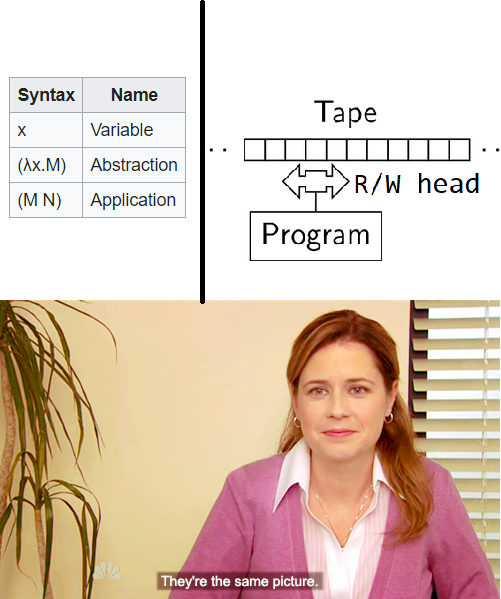
\includegraphics[scale=.35]{images/same_thing.png}
\end{column}
\end{columns}
\end{frame}

%------------------------------------------------
\begin{frame}{Lambda calcul în informatică}

\begin{center}

\includegraphics[scale=.35]{images/haskell.jpeg}
\end{center}

\begin{itemize}
	\item Lambda calcul este un limbaj de programare ideal.
	\medskip
	\item Probabil cel mai simplu limbaj de programare Turing complet.
	\medskip
	\item Toate \alert{limbajele de programare funcțională} sunt extensii ale lambda calculului cu diferite caracteristici (tipuri de date, efecte laterale etc)
\end{itemize}
\end{frame}

%------------------------------------------------
\begin{frame}{Proofs-as-programs}

\begin{itemize}
	\item \alert{Ce este o demonstrație}?
	\begin{itemize}
		\item \intens{Logica clasică}: plecând de la niște presupuneri, este suficient să ajungi la o contradicție
		\item \intens{Logica constructivistă}: pentru a arata ca un obiect există, trebuie să îl construim explicit.
	\end{itemize}
	\medskip 
	\item Legătura dintre lambda calcul și logica constructivistă este dată de paradigma \textit{\intens{proofs-as-programs}}.
	\begin{itemize}
		\item o demonstrație trebuie să fie o "construcție", un program
		\item lambda calculul este o notație pentru astfel de programe
	\end{itemize}
\end{itemize}

\end{frame}



%------------------------------------------------
\begin{frame}
  \vfill
  \centering

\textbf{\large \alert{Quiz time!}}


\includegraphics[scale=.35]{../Quiz/C01-Q1.png}

 \url{https://tinyurl.com/C01-Quiz1}
  \vfill
\end{frame}
%---------------------------------------------
\begin{frame}
  \vfill
  \centering

\textbf{Pe săptămâna viitoare!}

  \vfill
\end{frame}
\end{document}






